
% This is all AmNat stuff
\documentclass[11pt]{article}\usepackage[]{graphicx}\usepackage[]{color}
% maxwidth is the original width if it is less than linewidth
% otherwise use linewidth (to make sure the graphics do not exceed the margin)
\makeatletter
\def\maxwidth{ %
  \ifdim\Gin@nat@width>\linewidth
    \linewidth
  \else
    \Gin@nat@width
  \fi
}
\makeatother

\definecolor{fgcolor}{rgb}{0.345, 0.345, 0.345}
\newcommand{\hlnum}[1]{\textcolor[rgb]{0.686,0.059,0.569}{#1}}%
\newcommand{\hlstr}[1]{\textcolor[rgb]{0.192,0.494,0.8}{#1}}%
\newcommand{\hlcom}[1]{\textcolor[rgb]{0.678,0.584,0.686}{\textit{#1}}}%
\newcommand{\hlopt}[1]{\textcolor[rgb]{0,0,0}{#1}}%
\newcommand{\hlstd}[1]{\textcolor[rgb]{0.345,0.345,0.345}{#1}}%
\newcommand{\hlkwa}[1]{\textcolor[rgb]{0.161,0.373,0.58}{\textbf{#1}}}%
\newcommand{\hlkwb}[1]{\textcolor[rgb]{0.69,0.353,0.396}{#1}}%
\newcommand{\hlkwc}[1]{\textcolor[rgb]{0.333,0.667,0.333}{#1}}%
\newcommand{\hlkwd}[1]{\textcolor[rgb]{0.737,0.353,0.396}{\textbf{#1}}}%
\let\hlipl\hlkwb

\usepackage{framed}
\makeatletter
\newenvironment{kframe}{%
 \def\at@end@of@kframe{}%
 \ifinner\ifhmode%
  \def\at@end@of@kframe{\end{minipage}}%
  \begin{minipage}{\columnwidth}%
 \fi\fi%
 \def\FrameCommand##1{\hskip\@totalleftmargin \hskip-\fboxsep
 \colorbox{shadecolor}{##1}\hskip-\fboxsep
     % There is no \\@totalrightmargin, so:
     \hskip-\linewidth \hskip-\@totalleftmargin \hskip\columnwidth}%
 \MakeFramed {\advance\hsize-\width
   \@totalleftmargin\z@ \linewidth\hsize
   \@setminipage}}%
 {\par\unskip\endMakeFramed%
 \at@end@of@kframe}
\makeatother

\definecolor{shadecolor}{rgb}{.97, .97, .97}
\definecolor{messagecolor}{rgb}{0, 0, 0}
\definecolor{warningcolor}{rgb}{1, 0, 1}
\definecolor{errorcolor}{rgb}{1, 0, 0}
\newenvironment{knitrout}{}{} % an empty environment to be redefined in TeX

\usepackage{alltt}
\usepackage[sc]{mathpazo} %Like Palatino with extensive math support
\usepackage{fullpage}
\usepackage[authoryear,sectionbib,sort]{natbib}
\linespread{1.7}
\usepackage[utf8]{inputenc}
\usepackage{lineno}
\usepackage{titlesec}
\titleformat{\section}[block]{\Large\bfseries\filcenter}{\thesection}{1em}{}
\titleformat{\subsection}[block]{\Large\itshape\filcenter}{\thesubsection}{1em}{}
\titleformat{\subsubsection}[block]{\large\itshape}{\thesubsubsection}{1em}{}
\titleformat{\paragraph}[runin]{\itshape}{\theparagraph}{1em}{}[. ]\renewcommand{\refname}{Literature Cited}
% my addnl packages
\usepackage{geometry}
\usepackage{graphicx}
\usepackage[T1]{fontenc}
\usepackage[utf8]{inputenc}
\usepackage{authblk}
\usepackage{setspace}
\usepackage{amsfonts,amssymb,amsmath,hyperref}
\usepackage{float}
\usepackage{caption}
\usepackage{multirow}
\usepackage{hyperref}
\usepackage{wrapfig}
\usepackage{rotating}
\usepackage[usenames,dvipsnames]{xcolor}
\newcommand{\revise}[1]{{\color{Black}{#1}}}



%-------------------------------------------------------------------------

\title{Two-sex demography, sexual niche differentiation, and the geographic range limits of Texas bluegrass (\textit{Poa arachnifera})}
\author{Tom E.X. Miller$^{1,\ast}$ and Aldo Compagnoni$^{2,3}$} 
\date{}
\IfFileExists{upquote.sty}{\usepackage{upquote}}{}
\begin{document}
\maketitle
\noindent{} 1. Program in Ecology and Evolutionary Biology, Department of BioSciences, Rice University, Houston, TX 77005;
\noindent{} 2. Institute of Biology, Martin Luther University Halle-Wittenberg, Halle, Germany;
\noindent{} 3. German Centre for Integrative Biodiversity Research (iDiv), Leipzig, Germany;
\noindent{} $\ast$ Corresponding author; e-mail: tom.miller@rice.edu

\bigskip

\textit{Manuscript elements}: Figures~1--6, online appendices~A--C. Figure~2 and Figure~6 are to print in color.

\bigskip

\textit{Keywords}: demography; dioecy; intra-specific niche heterogeneity; matrix projection model; sex ratio; range limits.

\bigskip

\textit{Manuscript type}: Article. %Or e-article, note, e-note, natural history miscellany, e-natural history miscellany, comment, reply, invited symposium, or historical perspective.

\bigskip

\noindent{\footnotesize Prepared using the suggested \LaTeX{} template for \textit{Am.\ Nat.}}

%\linenumbers{}
%\modulolinenumbers[3]

\newpage{}

\section*{Abstract}
\linenumbers
Understanding the mechanisms that generate biogeographic range limits is a long-standing goal of ecology. 
It is widely hypothesized that distributional limits reflect the environmental niche, but this hypothesis is complicated by widespread potential for intra-specific niche heterogeneity. 
In dioecious species, sexual niche differentiation may cause divergence between the sexes in their limits of environmental suitability. 
We studied range boundary formation in Texas bluegrass (\textit{Poa arachnifera}), a perennial dioecious plant, testing the alternative hypotheses that range limits reflect the niche limits of females only versus the combined contributions of females and males, including their inter-dependence via mating. 
Common garden experiments across a longitudinal aridity gradient revealed female-biased flowering approaching eastern range limits, suggesting that mate limitation may constrain the species' distribution. 
However, a demographic model showed that declines in $\lambda$ approaching range limits were driven almost entirely by female vital rates. 
The dominant role of females was attributable to seed viability being robust to sex ratio variation and to low sensitivity of $\lambda$ to reproductive transitions.
We suggest that female-dominant range limits may be common to long-lived species with polygamous mating systems, and that female responses to environmental drivers may often be sufficient for predicting range shifts in response to environmental change.

%-------------------------------------------------------------------------
\section*{Keywords}
demography; dioecy; intra-specific niche heterogeneity; matrix projection model; sex ratio; range limits

%--------------------------------------------------------------------
\newpage
\section*{Introduction}

Understanding the processes that generate species' distributional limits is a foundational objective of ecology.
The niche concept is central to theory for range limits \citep{Hutchinson1958} and available evidence suggests that geographic distributions may often be interpreted as ecological niches ``writ large'' \citep{lee2016synthesis,hargreaves2013species}. 
Species distribution modeling has long capitalized on this idea to infer niche characteristics from statistical associations between occurrence and environmental variables.
In contrast, there is growing interest in process-based models of range limits, where individual-level demographic responses to environmental variation inform predictions about the ecological niche and environmental limits of population viability (i.e., at least replacement-level population growth, $\lambda \geq 1$) \citep{merow2014using,merow2017climate,diez2014probabilistic}. 
The mechanistic understanding offered by process-based models of range limits provides a potentially powerful vehicle for predicting range shifts in response to current and future environmental change \citep{evans2016towards,ehrlen2015predicting}. 

The widespread idea that range limits reflect niche limits intersects awkwardly with another pervasive concept in ecology: intra-specific niche heterogeneity. 
This refers to the fact that individuals within a population or species may differ in their interactions with the biotic and/or abiotic environment \citep{bolnick2002ecology,araujo2011ecological,holt2009bringing}. 
Intra-specific niche differences may correspond to demographic state variables such as life stage, size class or other, unmeasured aspects of individual identity. 
If range limits are a geographic manifestation of niche limits, but a single population or species may be comprised of many niches, then whose niche is it that determines the geographic distribution and how would we know?

Sexual niche differentiation is a common form of intra-specific niche heterogeneity \citep{bolnick2002ecology} and has been widely documented in animals (the vast majority of which are dioecious) and plants (ca. 6\% of angiosperms are dioecious: \citealt{renner1995dioecy}). 
The prevalence of sexual niche differentiation was recognized by Darwin (\citeyear{darwin2019descent}), who described ``different habits of life, not related...to the reproductive functions'' of females and males.
There are now many examples of sex differences in trophic position \citep{pekar2011intersexual,law2018carnivory}, habitat use \citep{bowyer2004sexual,phillips2004seasonal,de2018habitat}, and responses to climate \citep{petry2016sex,rozas2009sex,gianuca2019sex}, differences that may or may not be accompanied by sexual dimorphism. 
It has been hypothesized that sexual niche differentiation may evolve by natural selection when it reduces competitive or other antagonistic interactions between the sexes \citep{bolnick2003sexual,de2015ecological}, as a byproduct of naturally or sexually selected size dimorphism \citep{shine1989ecological,temeles2010evolution}, or when females and males pay different costs of reproduction \citep{bierzychudek1988spatial}.

Sexual niche differentiation can translate to sex-specific \revise{demographic} advantages in different environments, causing skew in the operational sex ratio (OSR: relative abundance of females and males available for mating) even if the primary (birth) sex ratio is unbiased \citep{veran2009demographic,shelton2010origin,eberhart2017sex}.
Indeed, environmental clines in OSR have been widely documented in plants and animals at fine spatial scales \citep{eppley2001gender,bertiller2002spatial,groen2010sex,hultine2018does,bisang2020sex} as well as broader climatic clines across alititutdes or latitudes \citep{petry2016sex,ketterson1976geographic,caruso2007sex,dudaniec2021latitudinal}. 
At range margins, where environments \revise{\linelabel{r1.1}may be} extreme relative to the range core,
demographic differences between the sexes, and hence skew in the OSR, may be greatest. 
In dioecious plants, for example, populations at upper altitudes and latitudes and in the more xeric margins of species' ranges tend to be male-biased, \revise{\linelabel{resources}possibly due to the greater resource demands of female flower and seed production} \citep{field2013ecological}.

Returning to the question of whose niche determines range limits given the potential for sexual niche differentiation, classic ecological theory assumes the answer. 
``Female dominance'' is a pervasive, often implicit feature of population-dynamic models whereby male availability is assumed to have no influence on female fertility \citep{miller2011confronting,rankin2007males,caswell1986two}. 
This assumption is wrong, of course, but it may be \emph{adequate} when the sex ratio is balanced or exhibits little variation. 
The female-dominant perspective predicts that female responses to environmental variation should govern range limits (Fig. \ref{fig:concept}). 
However, females may be mate-limited in environments in which they are favored, which could reduce population viability in marginal environments \revise{\linelabel{marginal}that are more suitable for females than males}. 
This creates an additional, ``two-sex'' pathway by which environmental drivers may set distributional limits, via perturbations to the mating pool that arise from sex-specific responses to the environment (Fig. \ref{fig:concept}). 
%While sexual niche divergence sets the stage for two-sex dynamics to play an important role in marginal environments, this influence may be dampened in mating systems where single males can fertilize many females \citep{miller2011sex} or in life histories where population viability is weakly sensitive to female fertility \citep{franco2004comparative}. 

Here we ask whether female demographic responses to environmental variation, alone, are sufficient to understand the ecological origins of range limits, or whether males and female-male interactions must additionally be considered. 
As an experimental model, we worked with a dieocious plant species (Texas bluegrass [\textit{Poa arachnifera}]) narrowly distributed across the sharp longitudinal aridity gradient of the southern Great Plains, US (Fig. \ref{fig:map}). 
%The environmental isocline governing aridity in this region is expected to shift eastward under climate change \citep{karl2009global}, so understanding how it sets distributional limits may aid in forecasting future range shifts. 
We hypothesized that sexual niche differentiation with respect to longitudinal variation in aridity may lead to skewed sex ratios approaching range limits, and that mate limitation at environmental extremes could cause range boundaries to deviate from female-dominant expectations. 

This study was conducted in four parts. 
First, we conducted surveys to ask whether natural populations of Texas bluegrass exhibit longitudinal clines in operational sex ratio across  the aridity gradient. 
Second, we conducted a common garden experiment at 14 sites throughout the southern Great Plains to quantify sex-specific demography in variable abiotic environments. 
Third, we conducted a local sex ratio manipulation experiment to quantify how viable seed production by females responds to variation in OSR. 
Finally, we connected sex-specific demography with inter-sexual mating dynamics in a two-sex modeling framework to derive demographically-driven predictions for geographic limits of population viability ($\lambda \geq 1$). 
We analyzed the demographic model to decompose the decline in $\lambda$ approaching range limits into contributions from female-dominant and two-sex pathways (Fig. \ref{fig:concept}).


%--------------------------------------------------------------------
\section*{Materials and methods}

\subsection*{Study system and natural population surveys}
\textit{Poa arachnifera} (Texas bluegrass) is a perennial, cool-season  grass endemic to the southern Great Plains. 
This species occurs almost exclusively in central Texas, Oklahoma, and southern Kansas (Fig. \ref{fig:map}) though there are occasional records of adventive populations in other U.S. states\footnote{http://bonap.net/Napa/TaxonMaps/Genus/County/Poa}.
\revise{\linelabel{rainfall}Seasonal rainfall in this region has two annual peaks, in spring and fall, which coincide with the growing-season of this C3 species.}
Like all grasses, \textit{P. arachnifera} is wind-pollinated.
Individuals can be sexed only when flowering, in early spring, based on the presence of stigmas (females) or anthers (males) in the inflorescence. 
Following inflorescence and seed production, plants go dormant for the hot summer months and vegetative growth resumes in fall. 
Individuals grow via rhizomes to form patches that may be as large as $50 m^2$ in area. 
Sex in \textit{P. arachnifera} is genetically based \citep{renganayaki2001genetic,renganayaki2005identification} and the primary sex ratio is $1$:$1$ (J. Goldman, USDA-ARS, \textit{unpubl. data}).
The rhizomatous growth habit allowed us to clonally propagate large numbers of known-sex individuals for experiments, as we describe below. 

We surveyed \textit{P. arachnifera} across its range to establish whether natural populations exhibited geographic clines in OSR corresponding to the longitudinal aridity gradient. 
We visited 14 populations in spring 2012 and 8 in spring 2013 (Table A1, Fig. \ref{fig:map}). 
At each location, we searched for \textit{P. arachnifera} along roads, trails, or creek drainages and recorded the number of female and male patches that we encountered and the number of inflorescences in each patch. \revise{\linelabel{season}We targeted our visits late in the flowering season to limit the influence of possible sex differences in phenology (inflorescences can be sexed after flowering is finished but not before it starts).}
To quantify the mating environment, we focus our analyses on the sex ratio of inflorescences rather than patches, since a single patch makes different contributions to the mating pool depending on whether it has few or many inflorescences. 

\subsubsection*{Statistical analysis of natural population surveys}
We fit a binomial generalized linear model (glm), where ``successes'' were female inflorescences and ``trials'' were total inflorescences, to test whether the OSR varied systematically with respect to longitude. 
Here and in the experiments that follow we use longitude as a proxy variable that captures all east-west environmental variation, notably precipitation (Fig. \ref{fig:map}) but also factors that co-vary with precipitation such as productivity. 
This statistical model and all those that follow were fit in a Bayesian statistical framework using Stan \citep{carpenter2017stan} and \textsf{R} package `rstan' \citep{stan2020rstan} with vague priors on all parameters.
In all cases, model fit was assessed with posterior predictive checks \citep{gelman1996posterior}. 

\subsection*{Common garden experiment}

\subsubsection*{Source material and experimental design}
We established a common garden experiment at 14 sites throughout and beyond the geographic distribution of \textit{P. arachnifera} (Fig. \ref{fig:map}, Table A2).
Experimental sites spanned latitudinal and longitudinal variation, though we focus here on longitude. 
During the three years of this experiment (2014--2017), total precipitation at each site closely tracked longitude (Fig. A1), as expected based on longer-term climate trends (Fig. \ref{fig:map}).
Source material for the experiment came from 8 sites, most of which were a subset of the sites that were visited for the natural population survey (Table A1, Fig. \ref{fig:map}). 
At these sites, we collected vegetative tillers from flowering individuals of each sex (mean: 11.6 individuals per site, range: 2--18). 
These were brought back to the Rice University greenhouse, where they were clonally propagated in ProMix potting soil and supplemented with Osmocote slow-release fertilizer at 78--80$^{\circ}$F under natural humidity and light. 

Common gardens were set up in Fall (October--December) 2014. 
At each site, we established 14 experimental blocks, which corresponded to a tree or woodland edge, providing partial shade that mimics this species' natural micro-environment. 
We planted 3 females and 3 males in each block, for a total of 42 individuals per sex per site and 1176 total plants across sites, with all source collections represented at all sites. 
Individuals were spaced within blocks to allow space for rhizomatous growth that could be clearly attributed to individual transplants. 
To promote establishment, we cleared vegetation immediately surrounding transplants and provided ca. $1$ L of water at the time of transplanting but provided no subsequent watering, fertilization, or competitor removal. 

We visited each site during May of 2015, 2016, and 2017. 
For each individual in each year, we recorded data for four demographic vital rates: survival status (alive or dead), size (number of tillers and patch area), flowering status (reproductive or vegetative), the number of panicles produced by flowering plants. %, and panicle length, which is proportional to production of seeds (in females) and pollen (in males). 

\subsubsection*{Statistical analysis of common garden experiment}
We analyzed the demographic vital rates with generalized linear mixed models in a hierarchical Bayesian framework. 
All the vital rates shared a common linear predictor for the expected value that included fixed effects of size, sex, linear and quadratic terms for longitude, and all 2- and 3-way interactions.
We included quadratic effects of longitude to account for the possibility of non-monotonic responses, following the hypothesis that fitness may peak in the center of the range. 
The linear predictor also included random effects of site, block, and source population of the transplant.
%; the corresponding variance terms were used in the demographic model (below) to capture process error in demography.  
We pooled all three years of observations for analysis so our results are implicitly averaged over years. 
\revise{\linelabel{waic}In Table B1, we used WAIC-based model selection (`loo' package: \cite{vehtari2017practical}) to show that vital rate models using precipitation and longitude as environmental covariates were statistically indistinguishable, which suggests that longitude is an adequate proxy for aridity.}

The survival and flowering data were Bernoulli distributed, and these models applied the logit link function. 
We modeled panicle counts as zero-truncated negative binomial using the log link. 
For growth, we modeled tiller number with a zero-truncated Poisson-Inverse Gaussian (PIG) distribution. 
For flowering and panicle production in year $t$, the size covariate was the natural logarithm of tiller number in year $t$. 
For survival and size in year $t$, the size covariate was the natural logarithm of tiller number in year $t-1$ (for 2015 data, size in year $t-1$ was transplant size at the time of planting). 
Posterior predictive checks indicated that these models described the data well (Fig. B1). 

\revise{\linelabel{mismatchmethods}In follow-up analyses, we tested the addition of a climate mismatch variable that quantified the deviation between mean annual precipitation of each source population and common garden location.
This analysis allowed us to evaluate whether local adaptation to climate may have contributed to variation in demographic performance across common garden sites. 
This was motivated by the observation that most source populations came from the interior of the geographic range and were brought to edge and beyond-edge locations that were much drier or wetter than their historical climate regime (Fig. \ref{fig:map}). 
The local adaptation hypothesis predicts that demographic performance declines with increasing climatic deviation between common garden and source population locations. 
To test this hypothesis we added the absolute value of mean annual precipitation mismatch (using 30-year normals) as a covariate to the vital rate models described above.}

\subsection*{Sex ratio experiment}
At one site near the center of the range (Lake Lewisville Environmental Learning Area, Texas), we established a separate experiment to quantify how sex ratio variation affects female reproductive success.
Details of this experiment, which was conducted in 2014--2015, are described in Compagnoni et al. \citeyear{compagnoni2017can}. 
Briefly, we established 124 experimental populations in $0.4 m \times 0.4 m$ plots that varied in population density (1--48 plants/plot) and sex ratio (0--100\%female), with 2--4 replicates for each of 34 density-sex ratio combinations. 
\revise{\linelabel{exp_source}We used plants from a single source population located ca. 200 km from the experimental site.} 
The experiment was established ca. 1 km from a natural population at this site and plots were situated with a minimum of 15 m spacing, a buffer that was intended to limit pollen movement between plots (pilot data indicated that $\geq 90\%$ of wind pollination occurred within $13 m$). 
We measured female reproductive success in different density and sex ratio environments by collecting panicles from a subset of females in each plot at the end of the reproductive season.
In the lab, we counted the total number of seeds on each panicle.

\revise{\linelabel{tzassay}In Texas bluegrass, unfertilized seeds shatter from the panicle along with fertilized seeds, so seed counts reflect female reproductive effort (seeds initiated) and not mating success (seeds fertilized). 
We therefore assessed seed fertilization in two ways. 
First, we conducted greenhouse-based germination trials using 25 seeds per panicle from 112 panicles belonging to 84 census females spanning the range of sex ratio variation. 
We also conducted tetrazolium-based seed viability assays to estimate seed fertilization independently of germination, since some fertilized seeds may fail to germinate during our trials.
Tetrazolium trials used 17--57 seeds per panicle (mode: 30) from 65 panicles belonging to 63 females, a subset of those used for the germination trials. To perform these assays, we first let seed batches imbibe on a moistened paper towel for 12 h. 
We then bisected the seeds in half and soaked them in a pH buffer solution containing 0.1\% of tetrazolium for 12 h. The pH buffer solution contained 0.57\% of sodium phosphate and 0.36\% of potassium phosphate. 
A seed was scored as viable if the embryo stained pink.}

\subsubsection*{Statistical analysis of sex ratio experiment}
Our previous study examined how interactions between density and frequency (sex ratio) dependence contributed to female reproductive success \citep{compagnoni2017can}. 
Here we focus solely on sex ratio variation, averaging over variation in density. 
Our goal was to estimate a `mating function' that defines how availability of male panicles affects the viability of seeds on female panicles.
We modeled the seed viability data with a binomial distribution where the probability of viability ($v$) was given by:

\begin{align}\label{eq:viab_fn}
v = v_{0} * (1 - OSR^{\alpha})
\end{align}

\noindent where $OSR$ is the operational sex ratio (fraction of panicles that were female) in our experimental populations. 
This function has the properties, supported by our previous work \citep{compagnoni2017can}, that seed viability is maximized at $v_{0}$ as $OSR$ approaches zero (strongly male-biased) and goes to zero as $OSR$ approaches $1$ (strongly female-biased).
Parameter $\alpha$ controls how viability declines with increasing female bias. 

We modeled germination data from greenhouse trials similarly, where counts of germinants were modeled as binomial successes.
Since germination was conditional on seed viability, the probability of success was given by the product $v*g$, where $v$ is a function of $OSR$ (Eq. \ref{eq:viab_fn}) and $g$ is assumed to be constant. 
The germination trials alone do not provide enough information to independently estimate $v$ and $g$ but the combination of viability and germination data allowed us to do so. 
For both viability and germination, we found that accounting for overdispersion with a beta-binomial response distribution improved model fit. 

\subsection*{Demographic model of range limits}
The statistical models for the common garden and sex ratio experiments provided the backbone of the full demographic model, a matrix projection model (MPM) structured by size (tiller number) and sex. 
Following the statistical modeling, the MPM accommodates longitude as a predictor variable, allowing us to identify the longitudinal limits of population viability ($\lambda \geq 1$) and investigate the underlying drivers of population decline at range limits. 

For a given longitude, let $F_{x,t}$ and $M_{x,t}$ be the number of female and male plants of size $x$ in year $t$, where $x \in \{1,2,...,U\}$ and $U$ is the maximum number of tillers a plant can attain (set to the 99th percentile of observed maximum size). 
We also include additional state variables for new recruits, $F^{R}_{t}$ and $M^{R}_{t}$, which we assume do not reproduce in their first year.
For ease of presentation, we do not symbolically show longitude effects in the vital rate functions for growth, survival, flowering, and panicle production but these all included longitude effects on the intercept and slope (with respect to size) as a second-order polynomial, following the statistical models.
We assume that the parameters of sex ratio-dependent mating (Eq. \ref{eq:viab_fn}) do not vary with longitude. 

For a pre-breeding census, the expected numbers of recruits in year $t+1$ is given by:

\begin{align}\label{eq:recruits}
F^{R}_{t+1} = \sum_{x=1}^{U} 	[ \, p^{F}(x) \cdot c^{F}(x) \cdot d \cdot v(\mathbf{F_{t}},\mathbf{M_{t}}) \cdot m \cdot \rho 	] \, F_{x,t}
\\
M^{R}_{t+1} = \sum_{x=1}^{U} 	[ \, p^{F}(x) \cdot c^{F}(x) \cdot d \cdot v(\mathbf{F_{t}},\mathbf{M_{t}}) \cdot m \cdot (1-\rho) 	] \, F_{x,t}
\end{align}

\noindent where $p^{F}$ and $c^{F}$ are flowering probability and panicle production for females of size $x$, $d$ is the number of seeds (fertilized or unfertilized) per female panicle, $v$ is the probability that a seed is fertilized, $m$ is the probability that a fertilized seed germinates, and $\rho$ is the primary sex ratio (proportion of recruits that are female). 
Seed fertilization depends on the OSR of panicles (following Eq. \ref{eq:viab_fn}) which was derived from the $U \times 1$ vectors of population structure $\mathbf{F_{t}}$ and $\mathbf{M_{t}}$:

\begin{align}\label{eq:viab_MPM}
v(\mathbf{F_{t}},\mathbf{M_{t}}) = v_{0} * \left[ 1 - \left( \frac{\sum_{x=1}^{U} p^{F}(x) c^{F}(x) F_{x,t}}{\sum_{x=1}^{U} p^{F}(x) c^{F}(x) F_{x,t} + p^{M}(x) c^{M}(x) M_{x,t}} \right) ^{\alpha}\right]
\end{align}

Finally, the dynamics of the size-structured component of the population are given by:

\begin{align}\label{eq:dynamics}
F_{y,t+1} = [ \, \sigma \cdot g^{F}(y,x=1) ] \, F^{R}_{t} + \sum_{x=1}^{U} 	[ \, s^{F}(x) \cdot g^{F}(y,x)] \, F_{x,t}
\\
M_{y,t+1} = [ \, \sigma \cdot g^{M}(y,x=1) ] \, M^{R}_{t} + \sum_{x=1}^{U} 	[ \,  s^{M}(x) \cdot g^{M}(y,x) ] \, M_{x,t}
\end{align}

\noindent For both females and males, the first term represents seedlings that survived their first year and enter the size distribution of established plants.
Because our common garden experiment relied on greenhouse-raised transplants we had little information on these early life cycle transitions, \revise{\linelabel{model}and filling these gaps was important for generating realistic predictions from the demographic model}. 
We used the seedling survival probability ($\sigma$) from our demographic studies of the hermaphroditic, perennial congener \textit{Poa autumnalis} in east Texas (T.E.X. Miller and J.A. Rudgers, \textit{unpublished data}) as a stand-in for \textit{P. arachnifera}, and we assume this probability was constant across sexes and longitudes (posterior mean $\sigma = 0.09$). 
We also assume that surviving seedlings reach size $y$ with probability $g(y,x=1)$, the expected future size of 1-tiller plants from the transplant experiment. 
The second term represents survival and size transition of established plants from the previous year, where $s$ and $g$ give the probabilities of surviving at size $x$ and growing from sizes $x$ to $y$, respectively, and superscripts indicate that these functions may be unique to females ($F$) and males ($M$). 

Because the two-sex MPM is nonlinear (vital rates affect and are affected by population structure) we estimated the asymptotic geometric growth rate ($\lambda$) by numerical simulation, and repeated this across a range of longitudes.
We used a regression-style Life Table Response Experiment \citep{caswell2001} to decompose the change in $\lambda$ towards range limits into contributions from female and male vital rates (the female-dominant hypothesis predicts that declines in $\lambda$ at range limits are driven solely by females). 
The LTRE approximates the change in $\lambda$ with longitude as the product of the sensitivity of $\lambda$ to the parameters times the sensitivity of the parameters to longitude, summed over all parameters:

\begin{align}\label{eq:ltre}
\frac{\partial \lambda}{\partial Longitude} \approx \sum_{i} \frac{\partial \lambda}{\partial \theta^{F}_{i}} \frac{\partial \theta^{F}_{i}}{\partial Longitude} + \frac{\partial \lambda}{\partial \theta^{M}_{i}} \frac{\partial \theta^{M}_{i}}{\partial Longitude}
\end{align}

\noindent Here, $\theta^{F}_{i}$ and $\theta^{M}_{i}$ represent sex-specific parameters: the regression coefficients for the intercepts and slopes of size-dependent vital rate functions. 
Because LTRE contributions are additive, we summed across vital rates to compare the total contributions of female and male parameters. 
Finally, we compared the two-sex MPM to the corresponding female-dominant model (Fig. \ref{fig:concept}B) by setting $v(\mathbf{F_{t}},\mathbf{M_{t}}) = v_{0}$, which decouples female fertility from the composition of the mating pool. 

%--------------------------------------------------------------------
\section*{Results}

\subsection*{Sex ratio variation in natural populations}
We found wide variation in operational sex ratio (proportion of total panicles that were female) across 22 natural populations of \textit{P. arachnifera}, including female-only and male-only populations (Fig. \ref{fig:survey}A). 
There was a longitudinal trend to sex ratio variation, with male-biased panicle production in the \revise{xeric} western parts of the range and female-biased panicle production in the \revise{mesic} east. 

\subsection*{Geographic variation in sex-specific demography}
In year one, there was near-total mortality of transplants at three sites in the common garden experiment due to various catastrophes (a flood, a drought, a pack of voles); otherwise, there was high (\>95\%) establishment. 
There was strong longitudinal variation in demography, including sex-specific demographic responses that varied across vital rates and interactions between size, sex, and longitude. 
Where sex-specific demographic responses occurred, they were almost always in favor of females. 
In Fig. \ref{fig:vital_rates}, we show binned means of raw data and fitted vital rate models for four vital rates (rows) and three size classes (columns); size was discretized for visualization only. 
This figure also shows the posterior distributions for the difference between the sexes across longitudes. 

Annual survival probability was predicted to peak at western and eastern range edges and was lowest at intermediate longitudes (Fig. \ref{fig:vital_rates}A-C). 
There was a modest female survival advantage but only at the western range edge for large sizes. 
Other vital rates showed the opposite (and more expected) longitudinal pattern for most sizes, with peaks in the center of the range and declines at eastern and western edges. 
There was a female growth advantage for small sizes at western longitudes (Fig. \ref{fig:vital_rates}D-F).
The strongest sex difference was in the probability of flowering: females had a flowering advantage, especially for large sizes and at eastern longitudes (Fig. \ref{fig:vital_rates}G-I). 
Finally, panicle production by flowering plants was similar between the sexes for most sizes, though for the largest sizes there were advantages for males in the west and females in the east (Fig. \ref{fig:vital_rates}J-L). 

Sex differences in flowering and panicle production generated a longitudinal trend in the operational sex ratio of our common garden populations consistent with (but weaker than) the trend in natural populations: the fraction of total panicles that were female in our common gardens increased from west to east (Fig. \ref{fig:survey}B) even as the fraction of surviving plants that were female did not show a longitudinal trend (Fig. \ref{fig:survey}C).
Thus, in recapitulating the natural OSR pattern, the common garden experiment revealed that the longitudinal trend in the mating pool of natural populations was due to the reproductive niche of females extending farther east than that of males, and not to sex differences in mortality.

\revise{\linelabel{mismatchresults}For survival, flowering, and panicle production we did not find strong evidence for local adaptation based on the posterior distributions of the climate mismatch coefficient (Fig. B2A,C,D). 
However, climate mismatch negatively affected growth such that plants from populations whose mean annual precipitation strongly differed from that of the common garden location exhibited reduced growth (Fig. B2B). }

\subsection*{Sex-ratio dependent seed fertilization}

Seed \revise{\linelabel{fert}fertilization} declined with increasing female bias in the sex ratio manipulation experiment. 
Fertilization success was greatest for females that were rare in male-biased populations, where 75-80\% of initiated seeds were viable (Fig. \ref{fig:seed_viability}). 
Fertilization was robust to sex ratio variation until ca. 75\% of the panicles in a population were female, at which point fertilization strongly declined due to pollen limitation.
The fitted model specifies that seed fertilization goes to zero as female bias goes to 100\% (Eq. \ref{eq:viab_fn}), and this assumption was generally consistent with the experimental results, where the majority (63\%) of females from female-only populations produced zero viable seeds. 
The occasional production of viable seeds in female-only populations (Fig. \ref{fig:seed_viability}) likely reflects rare pollen contamination between experimental plots. 
 
\subsection*{Two-sex model of range limits}
The \revise{process-based} demographic model connected sex-specific vital rate responses to longitudinal variation (Fig. \ref{fig:vital_rates}) with sex ratio-dependent mating (Fig. \ref{fig:seed_viability}) to predict the contributions of females and males to range limitation. 
The model predicted maximum fitness in the center of the range and loss of population viability at longitudes that corresponded well with observed range limits. 
Specifically, the western-most and eastern-most county records of \textit{P. arachnifera} fell within the uncertainty distribution of the model's predictions (represented by the shading in Fig. \ref{fig:lambda_long}A), bolstering our confidence that the model effectively captured the demographic drivers of range limitation in this species. 
Also, the asymptotic population structure predicted by the model showed female bias in the operational (panicle) sex ratio toward the eastern range margins, consistent with observations from the common garden and natural populations (Fig. B5A). 
Female bias in the OSR was predicted to cause declines in seed viability toward eastern range margins (Fig. B5B).
However, this effect was weak in magnitude because predicted OSR bias was not extreme enough to cause strong declines in viability, given the relationship derived from the sex ratio manipulation experiment (Fig. \ref{fig:seed_viability}). 
Furthermore, population viability at the eastern range margin was weakly sensitive to seed viability relative to other vital rates (Fig. B5C). 
These observations underscore the next set of results. 

LTRE decomposition revealed that declines in $\lambda$ approaching range limits were driven almost exclusively by females (Fig. \ref{fig:lambda_long}B) with near-zero contributions from males (Fig. \ref{fig:lambda_long}C). 
Thus, range limitation was an effectively female-dominant process, despite systematic geographic variation in sex ratio. 
Correspondingly, predictions of the two-sex model were nearly indistinguishable from a corresponding female-dominant model with all else equal, with only very modest differences in predictions of the two models emerging in the eastern part of the range (Fig. B4). 

Decomposition analysis further revealed that multiple female vital rates contributed to range limits, some in opposing directions. 
Because female survival increased toward range limits (Fig \ref{fig:vital_rates}A-C), this vital rate had a contribution to $\frac{\partial \lambda}{\partial Longitude}$ that was opposite in sign to the other vital rates (Fig. \ref{fig:lambda_long}B). 
However, increased survival at range edges was not sufficient to offset declines in other vital rates. 
The overall decline in $\lambda$ was driven most strongly by a combination of reduced flowering and growth in females at both the eastern and western limits (Fig. \ref{fig:lambda_long}B). 

Skew in the OSR predicted by the demographic model was less extreme than was observed in natural and experimental populations (Fig. B5A). 
This occurred because sex differences in demography, especially flowering, were most pronounced at the largest sizes, and the MPM predicted that these sizes were very rare at stable population structure. 
The stable size distribution predicted by the MPM corresponded well to the common garden data (from which the MPM was built) but was much smaller, on average, than the size distribution we observed in natural populations (Fig. C2), presumably because transplants did not grow like ``real'' plants and/or did not have time in our three-year experiment to reach those sizes. 
In Appendix C, we explore whether higher growth rates, leading to a more realistic size distribution, would lead to a more important role for males.
In numerical experiments with growth parameters, we found that larger size distributions led to stronger female bias and thus stronger reductions in seed viability at eastern range margins (Fig. C3). 
While these changes increased the contributions of males to range limitation, female contributions were still more than twice as important as males, and there was very little difference between predictions of the two-sex and female-dominant models even under this elevated growth scenario (Fig. C4). 
This leads us to conclude that, while our common garden-parameterized model may quantitatively underestimate OSR bias and its demographic consequences relative to natural populations, our qualitative conclusion that range boundary formation is effectively female-dominant in this system is robust to any biases imposed by the growth trajectories and size distributions of common garden populations. 


%--------------------------------------------------------------------

\section*{Discussion}

Understanding the causes of decline in population viability at range edges is a classic ecological problem and the foundation for predicting how species' ranges will respond to global change drivers. 
Sexual niche differentiation has the potential to generate skew in the mating pool across environmental gradients and may therefore contribute to reproductive failure at range edges of dioecious species. 
In Texas bluegrass, we found evidence for sexual niche differentiation that manifested over a large-scale geographic gradient: the female reproductive niche (environment-dependent flowering and panicle production) extended farther east than that of males, generating female-biased operational sex ratios toward the eastern, mesic range margins, a pattern detected in natural populations and recapitulated in our common garden populations. 
Furthermore, seed viability declined with increasing skew in the OSR, indicating that mate (pollen) limitation can limit the reproductive output of female-biased mating pools. 
It would appear that all the pieces are in place for an important role of two-sex dynamics in contributing to distributional limits of Texas bluegrass, particularly at the eastern range edge. 
Yet, insights derived from the field-parameterized population model indicate the opposite: range limitation in this species is an effectively female-dominant process, with negligible contributions from males. 
Thus, in this system and likely others, female dominance is an adequate framework for understanding range dynamics: despite evidence for sexual niche differentiation, only the female niche mattered for determining the environmental limits of population viability. 
This does not mean that sex is unimportant, but rather that lack of sex is never so severe that it limits population viability. 

The limited role of males in our experimental system can be explained by two factors. 
First, seed fertilization was robust to variation in OSR and was not predicted to strongly decline within the range of OSR bias that we observed and modeled, suggesting that few males are required to pollinate all or most females. 
Second, population growth ($\lambda$) was weakly sensitive to seed viability, which further buffered the demographic consequences of sex ratio bias. 
We speculate that our qualitative conclusions should apply to other species or systems that satisfy either, but especially both, of these conditions. 
While there are striking examples of female-biased sex ratios causing declines in population growth \citep{milner2003reproductive} or range expansion \citep{miller2013sex}, other examples suggest limited demographic consequences of sex ratio variation \citep{mysterud2002role,ewen2011demographic,gownaris2020sex}. 
Ultimately, sensitivity of female reproductive success to sex ratio should depend strongly on the mating system, with female dominance at the ``extremely polygamous'' end of a continuum \citep{miller2011sex}. 
The sensitivity of population viability to female reproductive success, in turn, is likely predicted by life history strategy: in long-lived, iteroparous species, population growth rates are often weakly sensitive to reproduction relative to growth and survival \citep{franco2004comparative}. 
We therefore hypothesize that range limits are more likely to be dominated by the female environmental niche in longer-lived species with more polygamous mating systems, while males are more likely to play an important role in shorter-lived, monogamous species that may be particularly sensitive to missed mating opportunities. 
As studies of sex ratio variation and sex-specific demography across species' ranges accumulate in the literature \citep[e.g.,][]{dudaniec2021latitudinal,petry2016sex,lynch2014climate}, this hypothesis may be tractably pursued with comparative analyses. 

While life history and mating system may determine the demographic consequences of skewed sex ratios, the sensitivity of sex ratio to environmental drivers is another critical ingredient of how environmental variation can affect the population dynamics of dioecious species.
Our study adds to a growing body of work quantifying the demographic mechanisms giving rise to skewed operational sex ratios using two-sex models \citep{eberhart2017sex,veran2009demographic,shelton2010origin} and parsing the contributions of environmental drivers \citep{bialic2020deer}.
%highlighting that OSR bias need not reflect differential mortality between the sexes \citep{ueno2007makes,morrison2016causes}. 
However, as a field, we lack a strong predictive framework for how often and in which direction environmental drivers are likely to skew the operational sex ratio -- and this gap is particularly important in the context of global change. 
We have focused on the limits of population viability with respect to geographic environmental variation but analogous processes will likely govern how populations respond to temporal environmental change (e.g., climate change), including direct effects on female demography and indirect effects via perturbations to the mating pool (Fig. \ref{fig:concept}). 
There is a need to better understand and predict which species and types of species are susceptible to climate change-induced shifts in OSR.
Geographic variation in OSR may be an instructive proxy for how dioecious species will respond to climate change \citep{petry2016sex}. 
The link between OSR and responses to climate adds value to studies of the causes and consequences of spatial variation in sex ratio, particularly at geographic scales that encompass ``past'' and ``future'' conditions. 

Previous studies of dioecious plants have shown that male bias is more common than female bias and is particularly pronounced in harsh abiotic environments, likely reflecting the greater resource requirements needed to pay the female cost of reproduction \citep{field2013comparative,field2013ecological,bierzychudek1988spatial}. 
Our surveys of natural populations are consistent with the broader pattern of male-biased OSR at xeric range edges.
However, our common garden populations did not exhibit \revise{strong} male bias in the xeric west -- averaged across years \revise{(Fig. \ref{fig:survey}B)} or in any single year (Fig. B3) -- nor did we find any strong demographic evidence for a western male advantage (in fact, there was a western female advantage in growth and survival for some sizes). 
\linelabel{males}If male advantage / female disadvantage under harsh abiotic conditions \revise{(suggested by the natural population trend: Fig. \ref{fig:survey}A)} is driven by the greater resource requirements of females then it is possible that clonal propagation and/or legacies of greenhouse rearing masked the `true' sex difference at xeric-edge common garden sites, \revise{\linelabel{r1.4}or that reproductive costs accumulate over longer time scales than considered here}. 
Instead, the stronger pattern of sex ratio bias was the female reproductive advantage at the mesic, eastern range edge. 
We hypothesize that the mesic edge is limited by competition and that the female reproductive advantage reflects competitive superiority of females, which has been suggested in previous studies of Texas bluegrass \citep{compagnoni2017can} and shown in other dioecious plants \citep{eppley2006females}, particularly under mesic conditions \citep{chen2014intra}. 
Theory suggests that biotic interactions such as competition are likely to limit species' ranges at the benign (e.g., mesic) end of abiotic gradients \citep{louthan2015and} though this has not been explored, to our knowledge, in the context of sex-structured dynamics.  
Future studies in our system or others could test whether females and males differ in their responses to biotic stressors at xeric and mesic range edges to reveal how biotic factors shape range limits via sex-specific demography.

Beyond the novel elements of sex-structured demography and mate limitation, our work informs and advances the broader literature on the processes generating species' range limits in at least three ways. 
First, the Texas bluegrass case study demonstrates that a process-based model capturing environment-dependent demography can accurately predict geographic range limits: the predicted limits of $\lambda \geq 1$ corresponded well to observed longitudinal limits from collection records, particularly given the uncertainty characterized by our hierarchical Bayesian statistical approach. 
We parameterized the model with respect to longitude, which tightly covaries with aridity in the southern Great Plains. 
Extensions of this model that transition from implicit to explicit consideration of aridity will allow us to forecast range responses of Texas bluegrass to future climate change and ask whether climate change will reduce or amplify OSR bias and mate limitation at longitudinal range edges. 
It would be interesting to additionally consider this species' latitudinal limits, though our exploratory analyses revealed no clear sex differences or sex ratio variation with respect to latitude. 

Second, our results also provide novel evidence for contrasting demographic responses to environmental drivers throughout a species' range -- or ``demographic compensation'' \citep{villellas2015demographic,doak2010demographic}. 
Elevated performance in some life history processes can compensate for declines in other processes and thus buffer range-edge populations against harsh environmental conditions. 
In Texas bluegrass, most vital rates declined toward eastern and western range limits but survival showed the opposite pattern. 
Increased survival at longitudinal extremes partially offset declines in other vital rates but this positive response was weaker than the negative responses.
Ultimately, increased survival was not sufficient to prevent declines in population viability from the range center to eastern and western limits, which were dominated by declining female growth and flowering. 
\revise{\linelabel{mismatchdiscussion}However, we also found evidence that growth patterns exhibited local adaptation: individuals planted into locations that were climatically similar to locations of their source population exhibited greater growth, on average, irrespective of sex. 
It is therefore possible that our demographic model (which does not explicitly account for local adaptation) over-estimates the decline in fitness approaching range edges, since local adaptation in a high-sensitivity vital rate may dampen the effects of environmental forcing. 
There is growing awareness that local adaptation can modify expectations for species' distributions under global change \citep{peterson2019incorporating}.
Mechanistic models of range limits that incorporate potential for local adaptation would be a valuable next step.}
%A recent study found a similar pattern, where compensation between vital rates could not prevent a decrease of population growth rate towards the southern range edge of \textit{Erythranthe cardinalis} \citep{sheth2018demographic}. 

Third, our results highlight some important considerations in how environment-dependent demographic models are best parameterized to derive insights into the drivers of range limits. 
Our approach relied heavily on common garden populations, which allowed us to plant and track known-sex individuals in contrasting environmental conditions that encompass and exceed the natural geographic distribution. 
The ability to robustly sample edge and beyond-edge environments is a powerful advantage of the common garden transplant approach \citep{hargreaves2013species}. 
However, this also limited the size variation that we were able to include and model, and the size distributions of common garden populations skewed consistently smaller than natural populations.
In Appendix C, we show that our conclusions are likely robust to this feature of the common gardens.
However, our ability to quantify the consequences of size representation is itself limited by size representation: we can simulate a population in which the largest common garden sizes are more common than they actually were, but simulating a population with sizes much larger than observed requires extrapolation of our statistical models, and we are skeptical about what insights such an exercise could provide (in Appendix C, we extrapolated demographic performance to sizes 50\% greater than the observed maximum). 
This issue is not unique to our study but will be encountered by any transplant study intended to yield inferences about range limits of species with significant size structure, such as trees.
If we could re-do our experiment knowing what we know now, we would combine data from natural and transplanted populations to model size-dependent demography over a more realistic size distribution.
Other investigators inspired by similar questions about the demographic drivers of range limits should consider such a hybrid approach.

\paragraph{Conclusion}
We have documented geographic variation in operational sex ratio; elucidated how sex-specific demographic responses to environmental drivers generate this pattern; quantified how female fertility responds to availability of males; and demonstrated that, in the end, sex ratio variation is a rather inconsequential component of declines in population viability at range limits. 
In Texas bluegrass and, we speculate, other dioecious plants and animals with similar life history and reproductive traits, the geographic distribution is essentially the \textit{female} environmental niche `writ large' \citep{hargreaves2013species}. 

Understanding and predicting geographic distributions and their responses to environmental change demands careful consideration of which biological details must be accounted for and which others can be safely ignored. 
Our results show that complex, non-linear dynamics involving females, males, and frequency-dependent reproduction can be reasonably approximated as a simple, linear process (female-dominant population growth).
We suggest that this is good news. 
The next challenge is to figure out how often and under what conditions ecologists can get away with it. 

%we have still no way to predict species whose OSR changes predictable across environmental gradients. We do have species-specific studies that explain the mechanisms that determine skewed OSR, such as sex differences in mortality \citep{meagher1981population}. However, there is no theory to predict dioecious species with environmentally controlled OSR.

%We used a plant model system for its powerful tractability (especially the opportunity to transplant known-sex individuals into contrasting environments) but it is worth considering how well insights from dioecious plants correspond to dioecious animals. 

%\begin{itemize}
%\item{Revisit conceptual importance of connecting niche heterogeneity with range limits.}
%\item{We found evidence for sexual niche differentiation.}
%  \begin{itemize}
%    \item{Common garden data indicated that females had a reproductive advantage at eastern limits. This recapitulated what we saw in natural population surveys.}
%  \end{itemize}
%\end{itemize}

%Our results suggest that in long-lived species with polygamous mating systems, range limits should reflect the niche limits of females. Polygyny implies mate limitation only at highly skewed sex ratios, and the population of long-lived species do not strongly depend on reproduction. Our polygynous model organism showed that mate limitation occurred became substantial only in populations comprised of 70\% females. Moreover, in long-lived species population growth rates will depend only weakly to reproduction \citep{franco2004comparative}.
%However, our results do not rule out the possibility that range limits are determined by both sexes in short-lived, polygynous species. 
%Because short-lived species are sensitive to reproduction, mate limitation will have substantial effects on their long-term population growth rate. 
%Mate limitation would therefore affect range limit formation when the OSR of a short-lived species changed dramatically across environmental gradients. 
%The literature provides several examples of short-lived species with environmentally controlled OSR \citep{freeman1976differential,freeman1985influence, purrington1993parental, eppley2001gender}. 

%However, the premises for males to contribute in range limit formation, albeit rare, are likely to occur in nature. First, female-skewed sex ratios are common both plants \citep{barrett2010ecological} and animals \citep{caswell2001}. Second, there are several examples of plants responding in contrasting ways to environmental gradients according to sex \citep{bierzychudek1988spatial}. These patterns can be driven by several mechanisms, such as physiology \citep{dawson1999sexual}, differences in competitive ability \citep{eppley2006females}, or demographic rates \citep{delph1999sexual}. Third, mate limitation is common in both animals \citep{gascoigne2009dangerously} and plants \citep{ashman2004pollen}. Accordingly, in plants, pollen limitation is considered the reason why dioecious plant species tend to have a substantially smaller range than selfing species \citep{grossenbacher2015geographic}.

%Despite demographic compensation, our evidence is consistent with the abundant center hypothesis of range formation. This hypothesis posits that the fitness and abundance of species will gradually decrease towards range edges \citep{brown1995spatial}. This is what our population model predicts, with maximum population growth rates at the center of the longitudinal gradient. However, to date the literature found mixed or contradictory evidence for this hypothesis. These previous tests relied on vital rates rather than population growth rates, providing contrasting results  \citep{sexton2009evolution,abeli2014effects}. As we show here, contrasting results among vital rates are expected, because demographic compensation is adaptive \citep{villellas2015demographic}. Accordingly, studies that calculate population growth rates along an environmental gradient tend to support the abundant center hypothesis. We know of four such studies in the existing literature, three of which showed a decrease in population growth rates towards at least one end of the environmental gradients \citep{eckhart2011geography,sheth2018demographic,baer2019declining}. %tom: I don't think that sheth 2018 supports abundant center; I am less familiar with the other two.
%The fourth study showed population growth rate along environmental gradients was unpredictable \citep{oldfather2019microclimate}.
% I wouldn't call these results `unpredictable'
%However, this last study emphasized the importance of microclimate, which can vary dramatically in alpine environments \citep{scherrer2010infra}. Hence, our results suggest that the abundant center hypothesis might hold in the studies that use population growth rate as response variable.

%--------------------------------------------------------------------
\section*{Acknowledgements}
We gratefully acknowledge the many individuals who facilitated our field work, especially Dariusz Malinowski, Jason Goldman, Tom Arsuffi, Alan Byboth, John Walker, Kenneth Steigman, Steven Gibson, Wesley Newman, Kerry Griffis, Liz Martin, Melanie Hartman, Brian Northup, Leland Russell, Dexter R Mardis, and Dixie Smith. 
This work was made possible by a network of biological field stations that hosted our geographically distributed experiment. 
We acknowledge Sam Houston State University, Texas A\&M University, University of Texas, Texas Tech University, Pittsburgh State University, and Wichita State University for investing in field stations and making these facilities available to us. 
We thank Marion Donald, Kory Kolis, Nakian Kim, and Alex Espana for valuable assistance in the field, lab, and greenhouse. 
The Geber Lab at Cornell University and two anonymous reviewers helped us improve our manuscript. 
Our work was supported by NSF Division of Environmental Biology awards 1543651 and 1754468 and by the Rice University Faculty Initiatives Fund. 

\section*{Author contributions}
A.C. and T.E.X.M. designed the study, carried out the study, and conducted the statistical analyses. 
T.E.X.M drafted the manuscript and both authors finalized the submission.

\section*{Data accessibility}
All data \citep{dryaddata} and code \citep{codepackage} are publicly available.

%--------------------------------------------------------------------
\newpage
\bibliographystyle{apalike}
\bibliography{POAR_range_limits}

\newpage

\begin{figure}
	\begin{center}
		%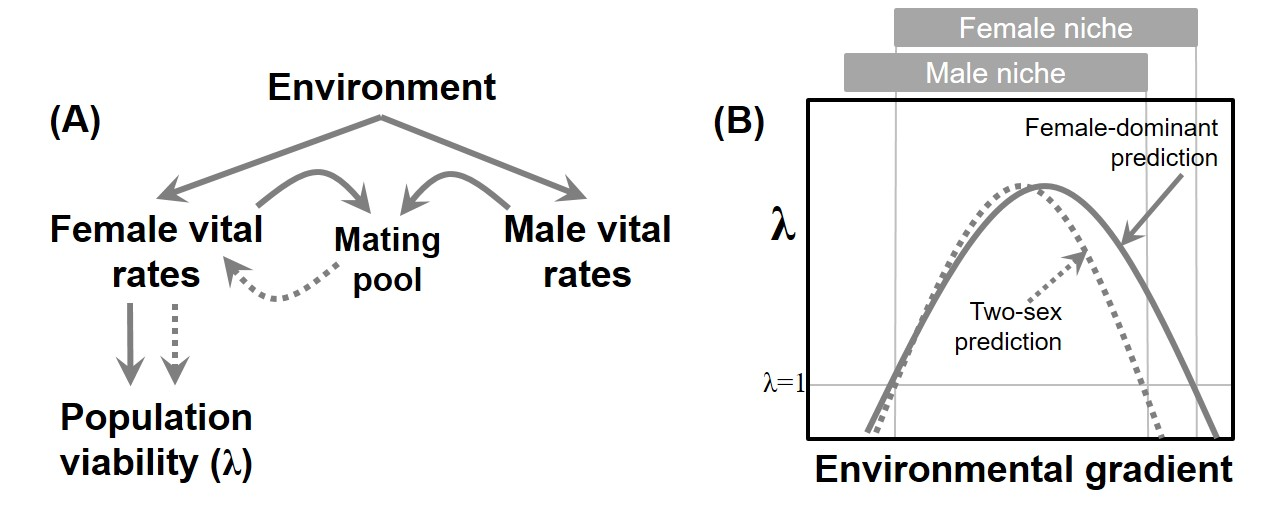
\includegraphics[width=0.95\linewidth]{Figures/conceptual_fig}
		\caption{Hypotheses for how environmental variation can affect population viability and range limits in dieocious species. 
			Under the female-dominant hypothesis, environmental drivers affect population growth ($\lambda$) through effects on females, alone (A). 
			In geographic / environmental space, this translates to range boundaries that arise at the limits of the female environmental niche, irrespective of where they fall with respect to the male niche (B). 
			Under the two-sex hypothesis, environmental drivers can affect $\lambda$ through sex-specific responses, which may skew the sex ratio of the mating pool and feed back to affect female fertility via mate availability (A). 
			In this case, expectations for range limits may differ from the female-dominant prediction, since mate limitation in environments that favor females over males may reduce population viability (B). 
			These are alternative hypotheses in the strict sense, but as the role of males becomes weaker the two-sex prediction converges on the female-dominant prediction.
		}
		\label{fig:concept}
	\end{center}
\end{figure}


\begin{figure}
	\begin{center}
%		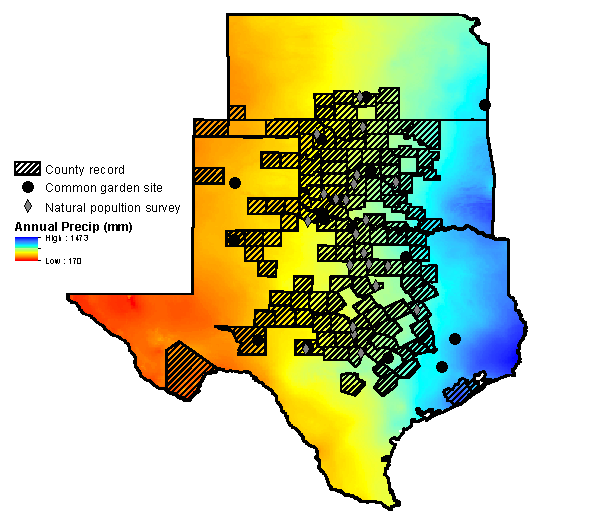
\includegraphics[width=0.75\linewidth]{Figures/POAR_BONAP_survey_garden_map}
		\caption{\revise{Geographic and environmental distribution of \textit{P. arachnifera} in Texas, Oklahoma, and Kansas. 
				Hatched shapes show counties with herbarium records of occurrence. 
				Color shows geographic variation in annual precipitation (mm) based on 30-year normals from WorldClim \citep{fick2017worldclim}. 
				Grey diamonds show natural population census locations, black points show sites for the common garden transplant experiment, and red points show locations of the source populations planted in each common garden site.}
		}
		\label{fig:map}
	\end{center}
\end{figure}


\begin{figure}
	\begin{center}
%		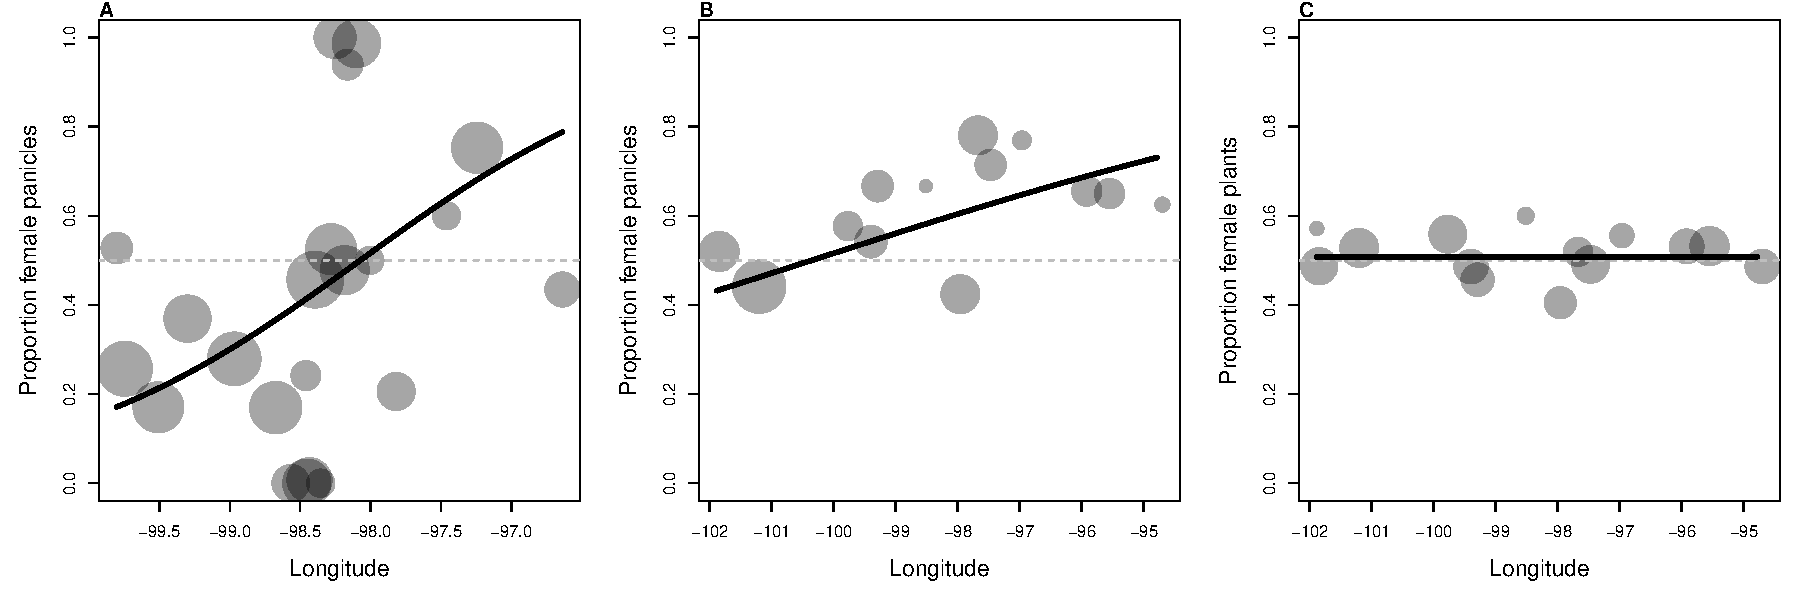
\includegraphics[width=1\linewidth]{Figures/nat_pops_gardens_SR}
		\caption{Sex ratio variation of \textit{P. arachnifera} across its longitudinal distribution.
			\textbf{A}, Operational sex ratio (fraction of panicles that were female) in 22 natural populations; \textbf{B}, Operational sex ratio and \textbf{C}, sex ratio (fraction of plants that were female) in 14 common gardens. 
			Within panels, point size is proportional to sample size (total number of panicles in \textbf{A,B} and total plants in \textbf{C}) as follows: \textbf{A}, min: 45, max: 2148; \textbf{B}, min: 1, max: 1021; \textbf{C}, min: 2, max: 79. 
			In \textbf{B,C}, data are pooled across years. 
			\revise{Gray lines show 500 samples from the posterior distribution of fitted binomial GLMs}.
		}
		\label{fig:survey}
	\end{center}
\end{figure}


\begin{figure}
	\begin{center}
%		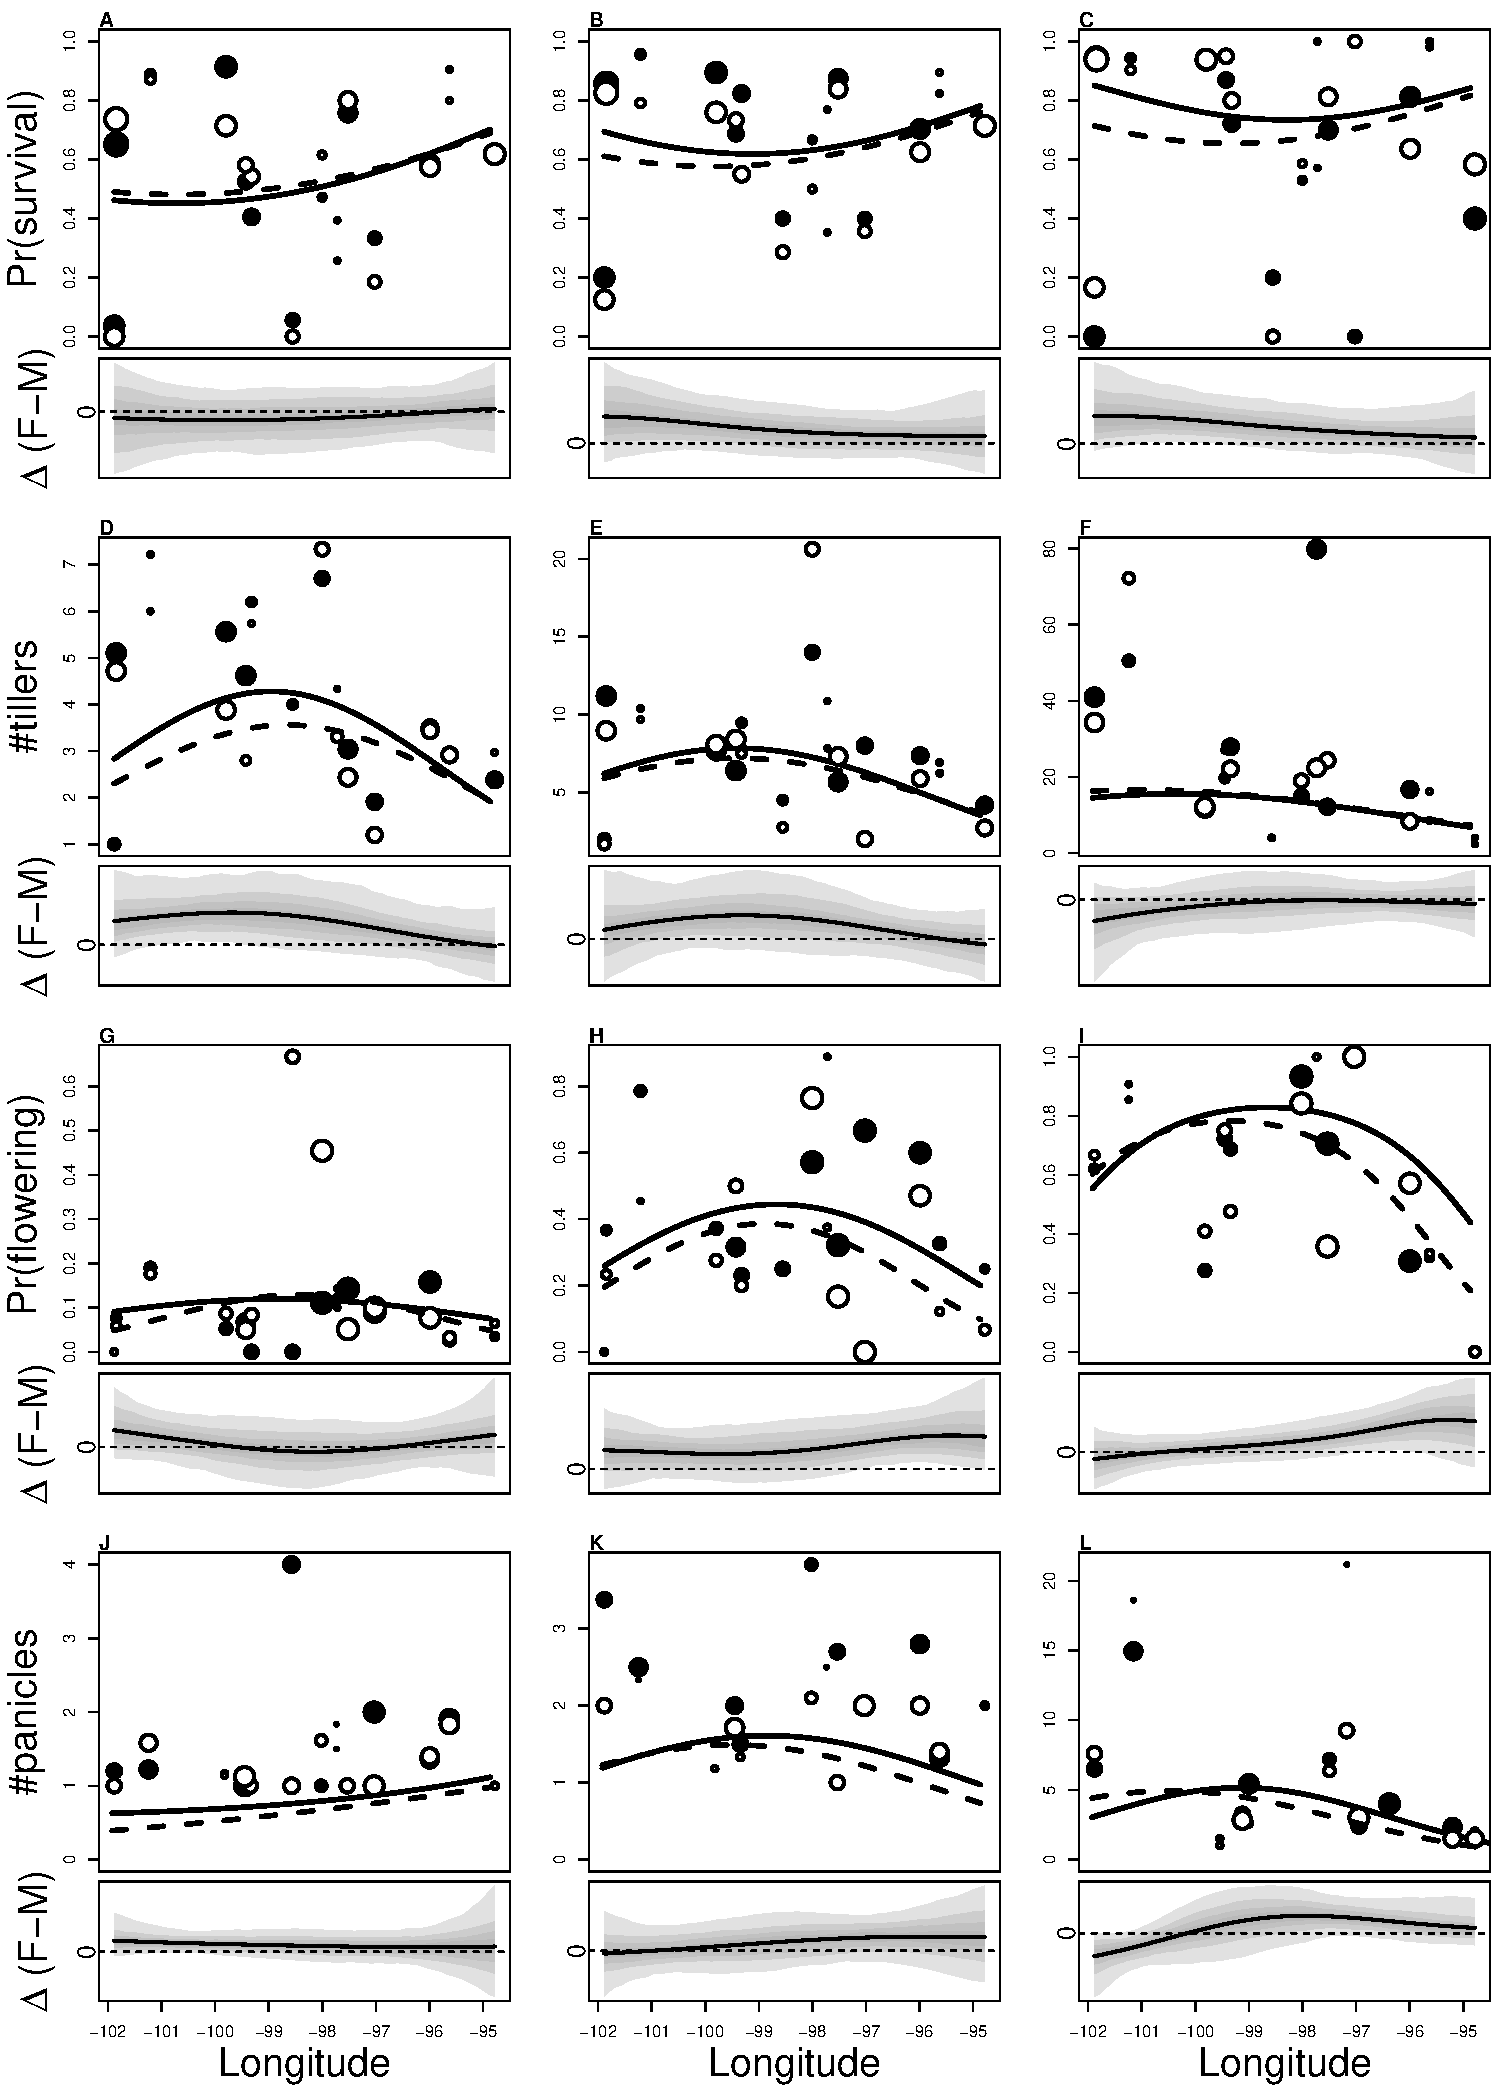
\includegraphics[width=0.85\linewidth]{Figures/vital_rates_v2}
		\caption{Sex-, size-, and longitude-related variation in:  A--C, inter-annual probability of survival; D--F, inter-annual growth (change in number of tillers); G--I, probability of flowering; J--L, number of panicles produced given flowering. 
			Points show means by site for females (filled) and males (open) and small (left column), medium (middle column), and large (right column) size classes (discretized, for visualization only).
			Point size is proportional to the sample size of the mean.
			Lines show fitted statistical models for females (solid) and males (dashed) based on posterior mean parameter values.
			Lower panels below each data panel show the posterior distribution of the difference between females and males as a function of longitude (positive and negative values indicate female and male advantage, respectively).
			\revise{Shaded contours show the 25, 50, 75, and 95 percentiles of the posterior distribution.}
			Dashed horizontal line shows zero difference.}
		\label{fig:vital_rates}
	\end{center}
\end{figure}


\begin{figure}
	\begin{center}
%		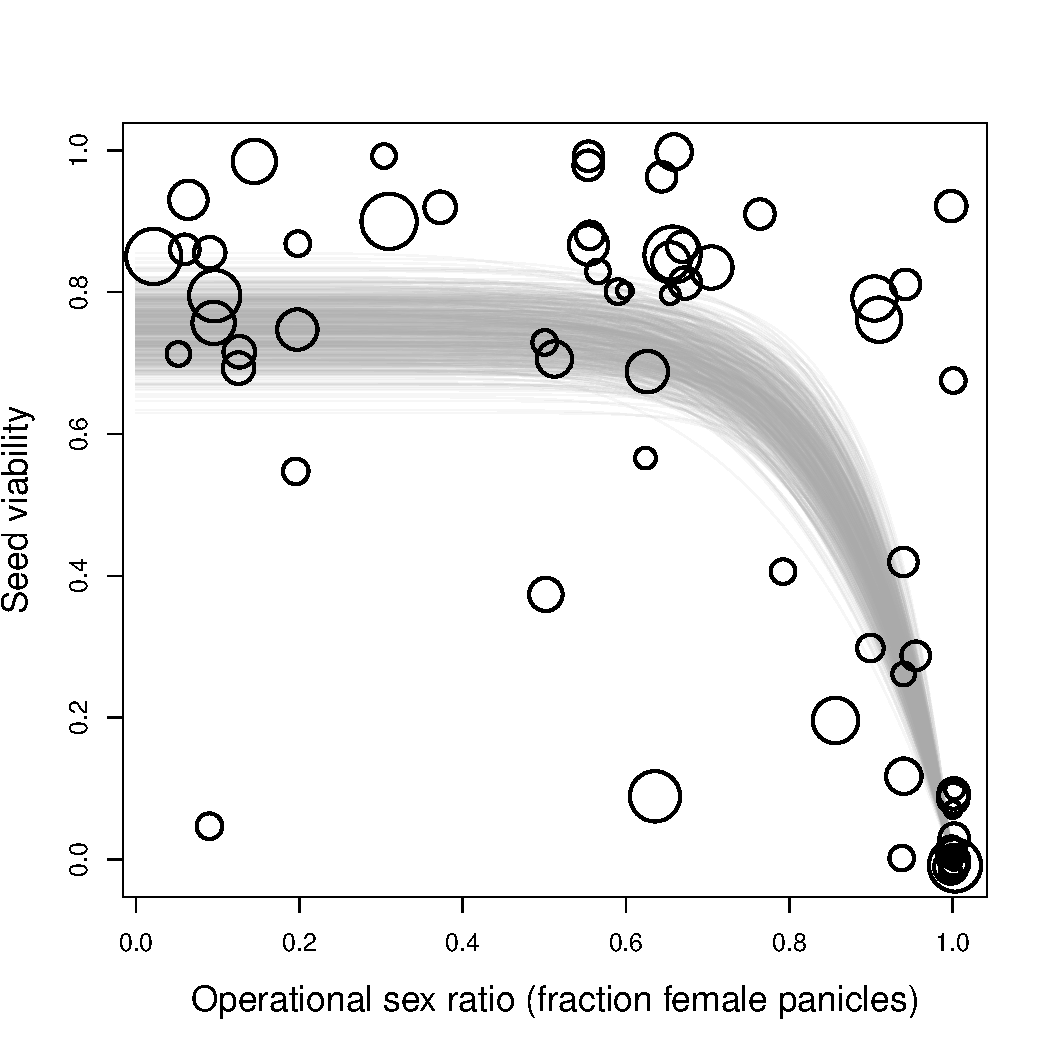
\includegraphics[width=0.6\linewidth]{Figures/seed_viability}
		\caption{Seed fertilization success in relation to operational sex ratio (fraction of panicles that are female) in experimental populations. 
			Circles show data from tetrazolium assays of seed viability; circle size is proprtional to the number of seeds tested (min: 14, max: 57).
			Lines show model predictions (Eq. \ref{eq:viab_fn}) for 500 samples from the posterior distribution of parameter estimates.}
		\label{fig:seed_viability}
	\end{center}
\end{figure}

\begin{figure}
	\begin{center}
%		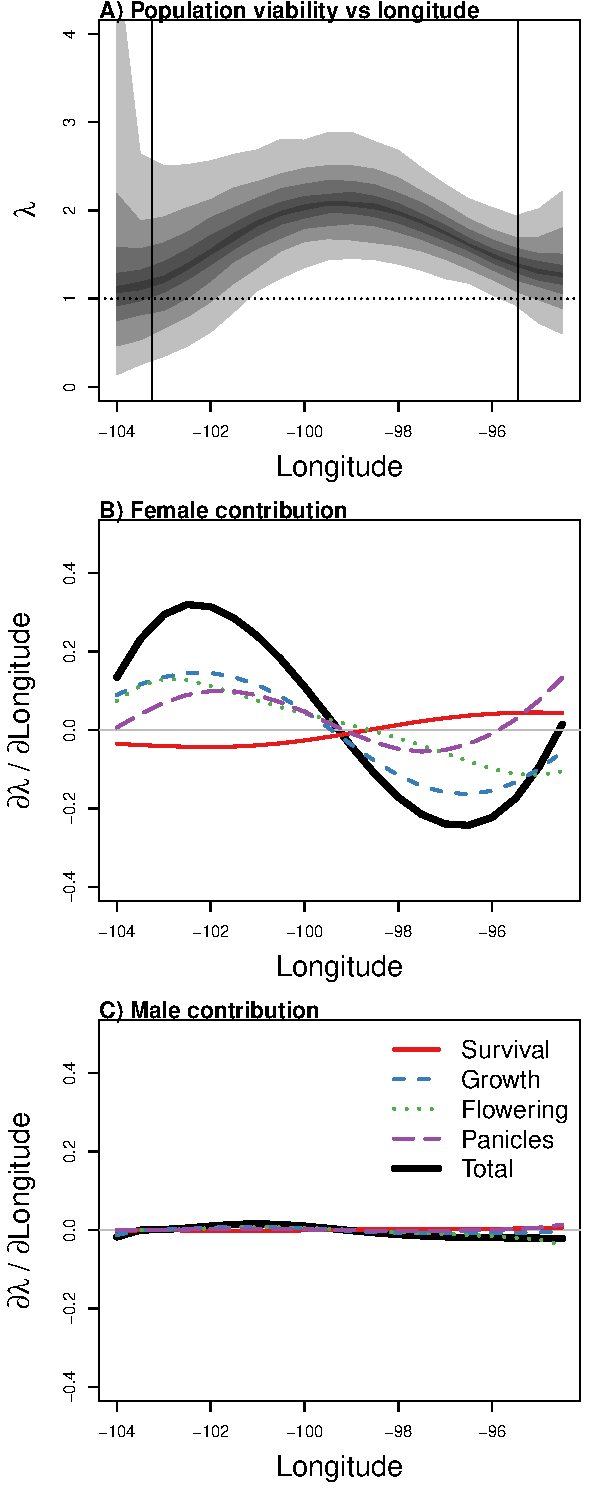
\includegraphics[width=0.5\linewidth]{Figures/lambda_long_ltre}
		\caption{Population growth ($\lambda$) as a function of longitude, predicted by the two-sex MPM that incorporates sex-specific demographic responses to longitude with sex ratio-dependent seed fertilization. 
			A, posterior distribution of $\lambda$, where shaded regions show the 25, 50, 75, and 95\% percentiles of parameter uncertainty. 
			Dashed horizontal line indicates the limit of population viability ($\lambda=1$) and vertical lines show the longitudes of Brewster and Brazoria Counties, TX, the western- and eastern-most occurrence records of \textit{P. arachnifera}.
			B--C, LTRE decomposition of the sensitity of $\lambda$ to longitude into additive vital rate contributions of females (B) and males (C) based on posterior mean parameter estimates. }
		\label{fig:lambda_long}
	\end{center}
\end{figure}





\end{document}
